\chapter{Interfaces}
\label{ch:Interfaces}
Defining the interfaces of this project is of great use in keeping track of all connections throughout the design, because insufficiently defining interface connections can lead to vast problems in the design phase.
Hence, an elaborate explanation and visual of interfaces is of great use through the help of a N2 chart and thereafter through software, communication, and hardware diagrams.

\section{N2 Chart}
\label{sec:N2Chart}
The N2 Chart defines the interfaces of the (sub)systems in the aerospace domain.
As can be seen from \Cref{fig:N2chart}, the N2 chart consists of the main subsystems in green, while surrounded by input and outputs.
In order to make the N2 Chart easily understandable, the typical clockwise input-to-output motion is used.
Hence, following this motion, the input and output of a certain system interface can be found.

To exemplify, one can take a look at the interface between Aerodynamics and Flight Performance,
where the inputs for Flight Performance are the aerodynamic coefficients and wing platform.
Thereafter it will output the cruise and stall speed, climb rate and angle, and flight envelope.
In return, these will be the inputs for the Aerodynamics systems,
which will output the new aerodynamic coefficients and wing platform again.
Therefore, the N2 Chart is of great use in defining the interfaces and having a clear overview of all interface connections at all times.

\begin{figure}[ht]
    \centering
    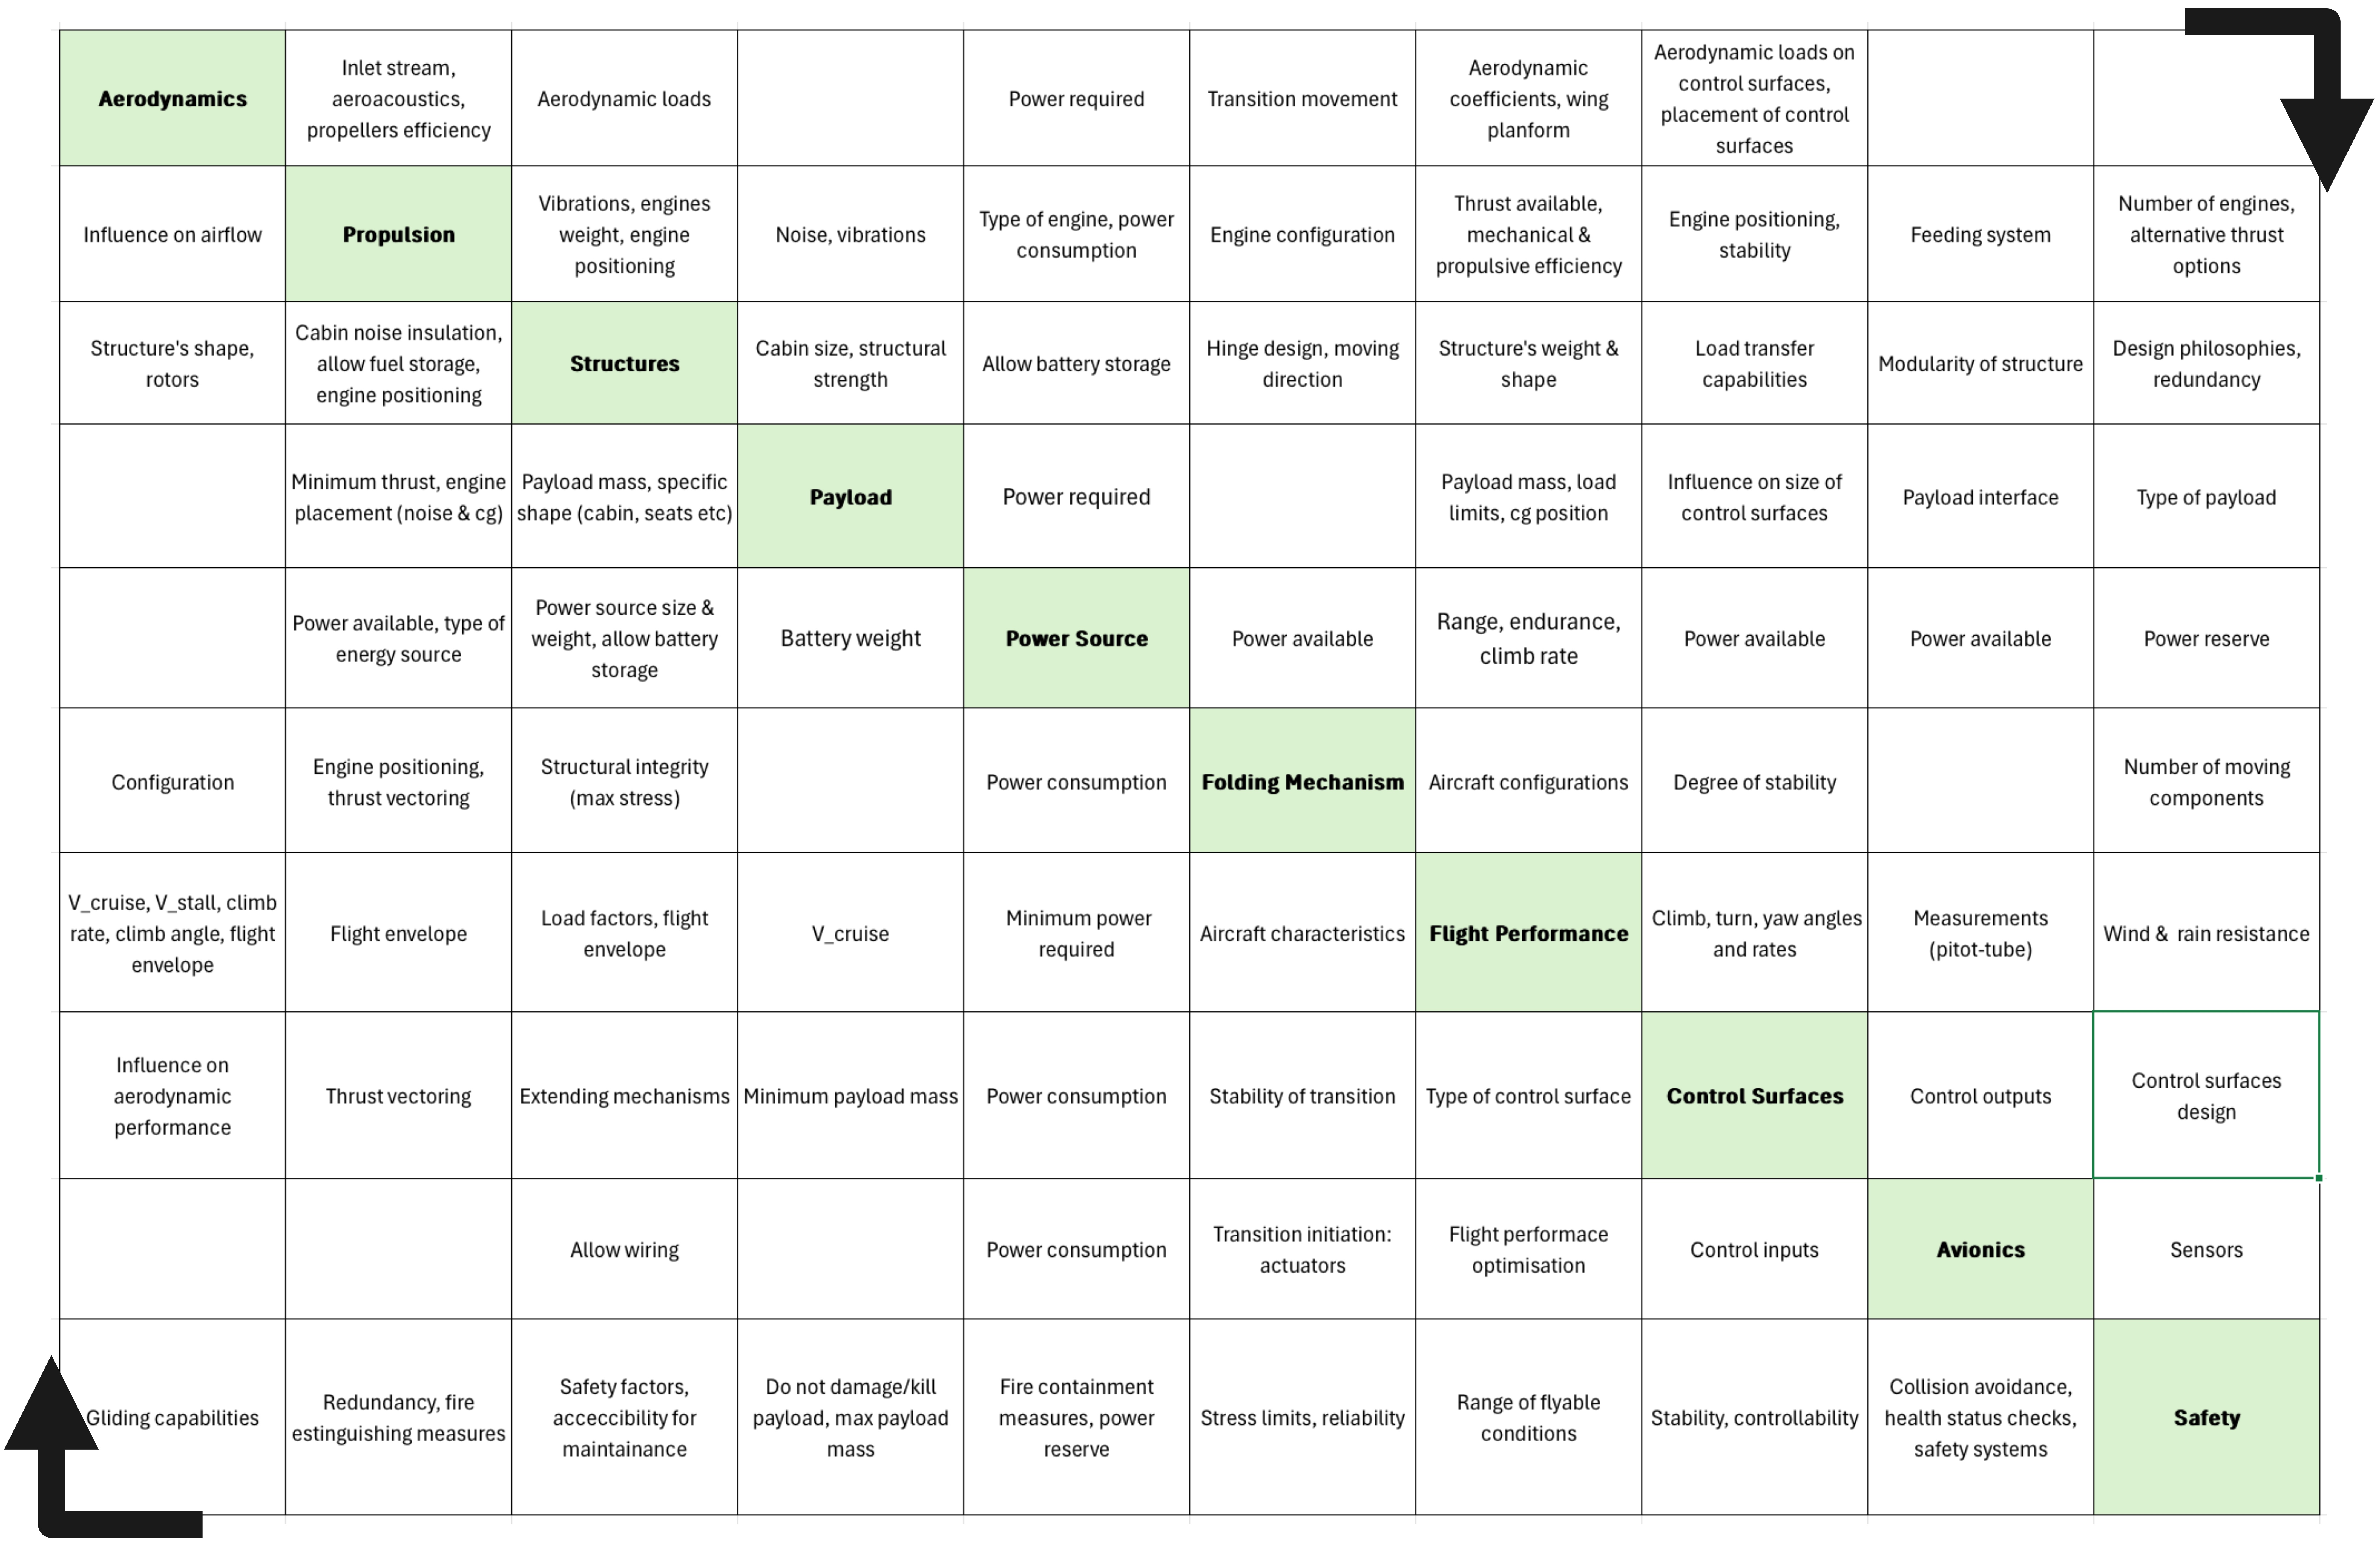
\includegraphics[width=1\linewidth]{figures/N2-chart.jpg}
    \label{fig:N2chart}
    \caption{N2 chart of (sub)systems}
\end{figure}

\section{Hardware Diagram}
\label{sec:HardwareDiagram}
In this section, the hardware components of the eVTOL are presented.
In particular, this is done visually via the diagram depicted on \Cref{fig:hwdiag}. In \Cref{tab:hwdiagacronyms} a list of acronyms with reference to \Cref{fig:hwdiag} can be found.
\begin{table}[H]
\centering
\caption{List of acronyms with reference to \Cref{fig:hwdiag}}
\label{tab:hwdiagacronyms}
\begin{tabular}{clcl}
\textbf{FCC} & Flight Control Computer    & \textbf{GNSS} & Global Navigation Satellite System \\
\textbf{VMS} & Vehicle Monitoring Sensors & \textbf{IMU}  & Inertial Measurement Unit          \\
\textbf{BMS} & Battery Management System  & \textbf{PDU}  & Power Distribution Unit           
\end{tabular}
\end{table}
\vspace{-5mm}
\begin{figure}[H]
    \centering
    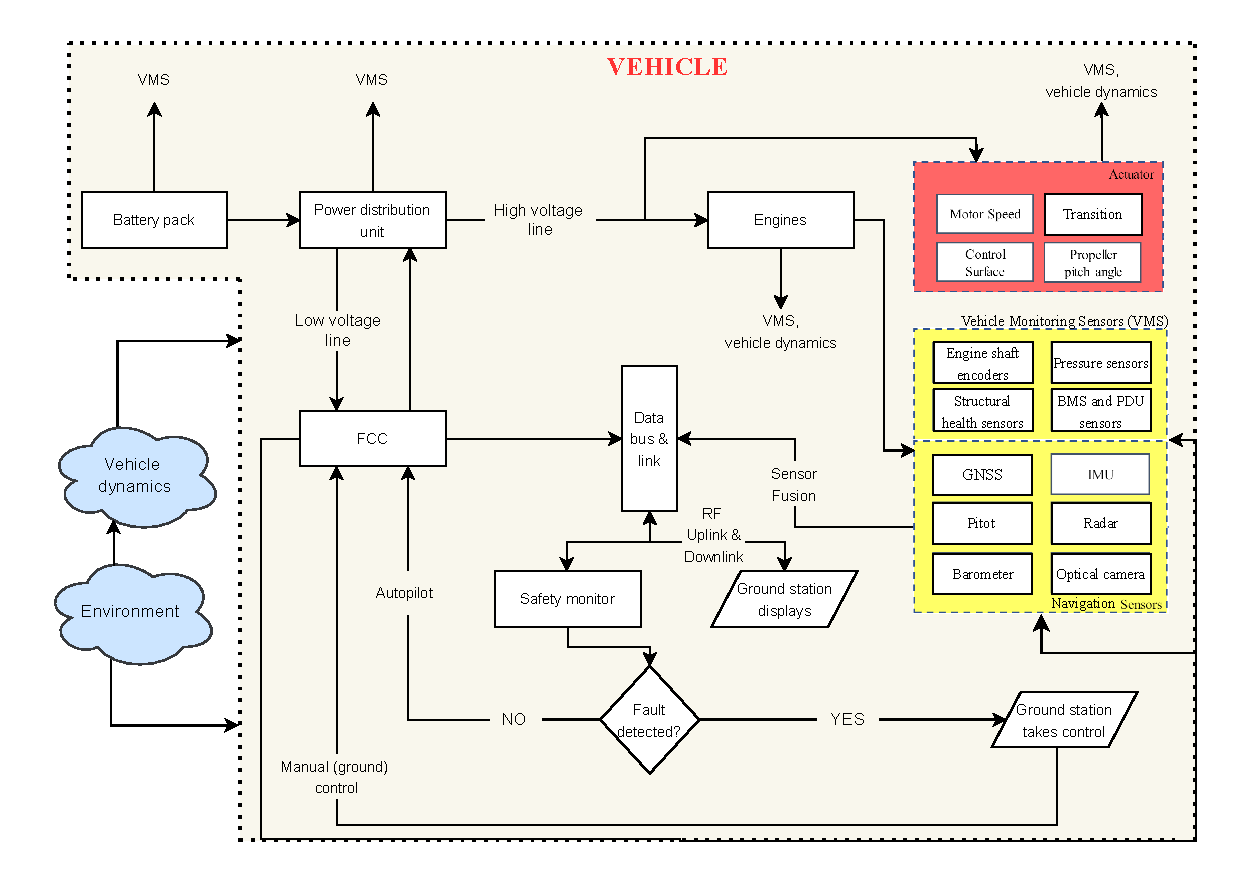
\includegraphics[width=\linewidth]{figures/HWdiagramUPDATED.pdf}
    \caption{H/W diagram}
    \label{fig:hwdiag}
\end{figure}
In \Cref{fig:hwdiag}, the main hardware components or groups are distinguished by white boxes, the actuation and sensor groups, given their diversity in composing parts, are instead grouped into the red and yellow frames respectively; lastly, sections of the diagram relative to the ground segment can be distinguished due to their parallelogram-shaped boxes.

\subsection{Diagram Flow Discussion}
The battery energy is managed by the PDU, which appropriately distributes it to the components of interest. The PDU follows orders from the FCC, which is the \enquote{brain} of the vehicle, where the main navigation, control and vehicle-handling software is located and executed. The orders outputted are based on the current power requirements and state of the vehicle.
Two power lines can be distinguished coming from the PDU, due to the substantially different power ($\text{power=}\text{voltage}\cdot \text{current}$) requirements: high- and low-voltage lines.
The high-voltage line powers the actuators and engines according to the thrust and attitude settings, dictated by the FCC, whereas the low-voltage line is connected directly to the FCC. The FCC, in turn, distributes the energy to all the low-power components in the vehicle, such as sensors.

The state of the aircraft is constantly monitored by a set of sensors measuring the state of the vehicle, speed, and attitude.
The actuators change the state and configuration, either hover or cruise, of the aircraft.
Sensor data is processed via sensor fusion algorithms, explained in \Cref{sec:SoftwareDiagram}, before being fed to the FCC for analysis.
A safety monitoring board is connected to the data bus, and if a critical functional flaw is detected, some action is taken.

It is finally important to underline the iterative nature of this diagram: in every cycle the vehicle responds to the environment and its dynamics via the actuators, which in turn leads to a change in vehicle dynamics, thus yielding a new set of commands. This is represented by those arrows ending on and coming from the dotted line, figuratively representing the vehicle update cycle iteration.

\subsection{Sensors}
A list of the sensors used is provided below, along with a rationale for each component (the unit numbers will be established in later design phases):
\begin{itemize}
    \item \textbf{Engine shaft encoders:} allowing for real-time determination of the RPMs per engine, and accurate thrust adjustments.
    \item \textbf{Pressure sensors:} allowing to measure and monitor, for instance, hydraulic pressures, pressure differential across the cabin, etc.
    \item \textbf{Structural health sensors:} group of sensors delegated to perform damage detection, event and monitoring (i.e., Mechanical Impact Diagnosis using passive piezoelectric sensors, impact damage diagnosis) \cite{hwdiagHEALTH}.
    \item \textbf{BMS} and \textbf{PDU sensors:} allowing for constant monitoring of battery and power lines health.
    \item \textbf{GNSS:} \enquote{providing positioning, navigation, and timing using navigational satellites from other networks beyond the GPS system}, \cite{gpsgov}.
    \item \textbf{IMU:} determines the specific angular rate, orientation of a body and force acting on it, using a combination of accelerometers, gyroscopes and magnetometers.
    \item \textbf{Pitot tube:} enables computation of the speed of the vehicle.
    \item \textbf{Radar:} allows for automated collision avoidance procedures.
    \item \textbf{Barometer:} allows for computation of the altitude of the vehicle.
    \item \textbf{Optical camera:} can transmit real-time footage back to the ground and allow for the implementation of computer vision algorithms.
\end{itemize}

\subsection{Actuators}
A list of the main actuators used is provided below, along with a rationale for each component (the unit numbers will be established in later design phases):
\begin{itemize}
    \item Control of \textbf{motor speed} and \textbf{control surfaces deflection angles} has a direct influence on the state of the vehicle, adapting it to its current settings.
    \item Actuation of \textbf{transition} mechanisms regulates the configuration change.
    \item Adjusting the \textbf{pitch angle} of the propellers mainly allows one to optimise the aircraft settings based on its current configuration.
\end{itemize}

\section{Software Diagram}
\label{sec:SoftwareDiagram}
The software configuration of the vehicle is depicted in \Cref{fig:SWdiagram}.
This schematic derives from the hardware diagram previously discussed and describes the parameters measured as well as the relations between the subsystems.

\begin{figure}[ht]
    \centering
    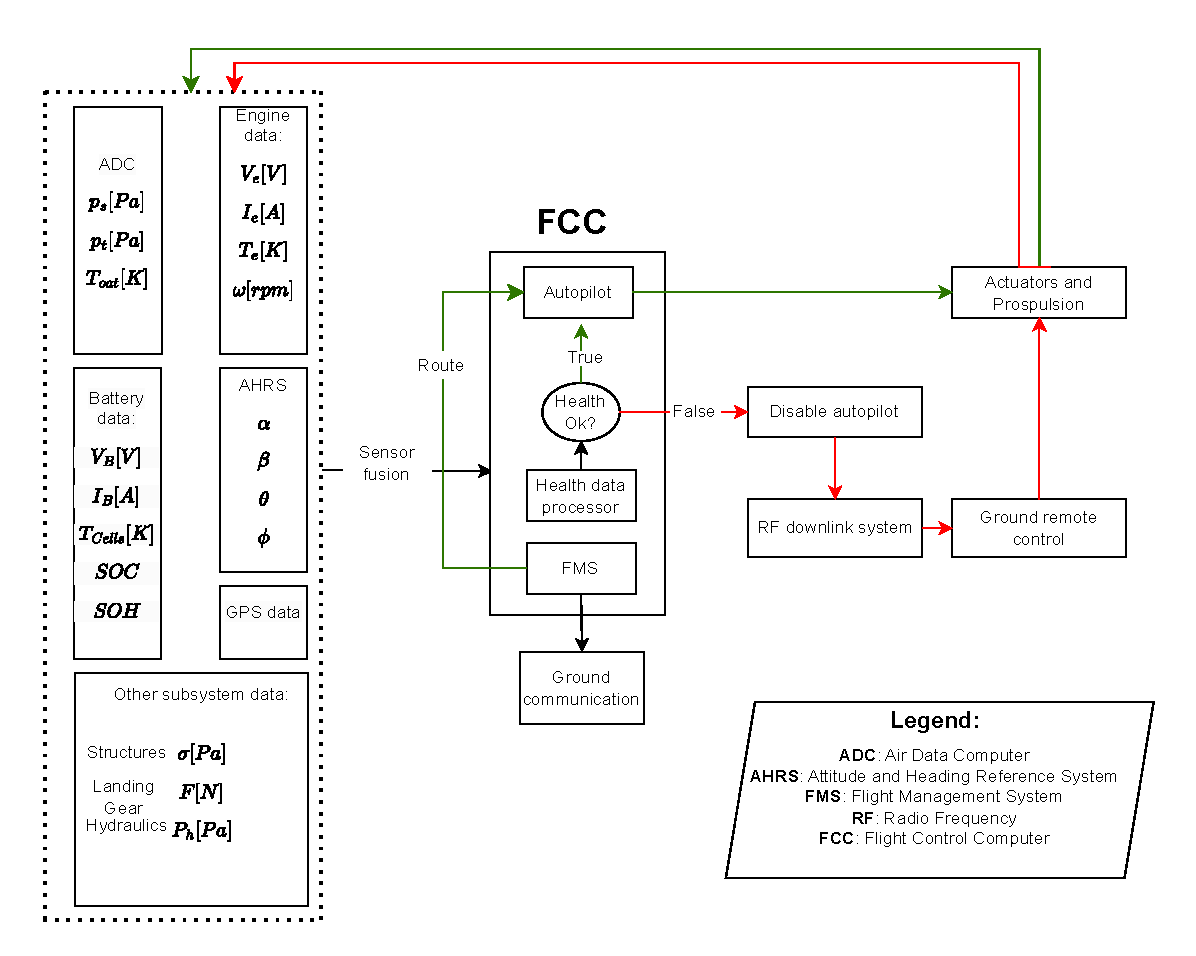
\includegraphics[width=0.9\linewidth]{figures/softwarediagramV2.pdf}
    \caption{Software diagram}
    \label{fig:SWdiagram}
\end{figure}

From the diagram, all the measured and computed parameters from the sensors can be seen. These are then transmitted to the flight control computer. Here, firstly, the health data are checked (i.e. Battery temperature), and if the test is passed, the autopilot will receive the parameters and follow the instructions of the FMS to pilot the eVTOL through the actuators and the propulsion system. In case the test is not passed, there is a downlink with a ground control station, which will take manual control and land the plane as soon as possible. This process is repeated as a loop, each and every moment in time only one of the two between the red and green branches in \Cref{fig:SWdiagram} will be followed, depending on the health condition.

In order to summarise all the parameters measured and used in the software diagram, table \Cref{tab:sensors} has been generated. Here, all the parameters are explained and the sensor measuring them is indicated, establishing the relation between software and hardware.


\begin{table}[H]
\centering
\caption{Measured parameters}
\label{tab:sensors}
\begin{tabular}{ccl|l}
\toprule
\multicolumn{3}{c|}{\textbf{Parameter}} & \textbf{Sensor Used}                \\ \midrule

$p_\text{s}, p_\text{t}$                & {[}Pa{]}                                        & (Static and total pressure)               & Pitot tube              \\
$T_\text{i}$                            & {[}K{]}                                         & (Air Temperature)                         & OAT sensor             \\
$V_\text{b}, V_\text{m}$                & {[}V{]}                                         & (Electric potential of battery and motor) & Voltometers      \\
$I_\text{b}, I_\text{m}$                & {[}A{]}                                         & (Electric current of battery and motor)   & Amperometers     \\
$\omega$                                & {[}rad/s{]}                                    & (Rotational speed)                        & Engine shaft encoder                     \\
SoC                                     & {[}\%{]}                                        & (State of charge)                         & Sensors in BMS                                     \\
SoH                                     & {[}\%{]}                                        & (State of health)                         & Sensors in BMS                                     \\
$\alpha$                                & {[}rad{]}                                       & (Angle of attack)                         & IMU                                      \\
$\beta$                                 & {[}rad{]}                                       & (Yaw angle)                               & IMU                                      \\
$\phi$                                  & {[}rad{]}                                       & (Roll angle)                              & IMU                                      \\
$\theta$                                & {[}rad{]}                                       & (Pitch angle)                             & IMU                                      \\
$\sigma$                                & {[}Pa{]}                                        & (Stresses on structures)                  & Strain gauges                           \\
$F$                                     & {[}N{]}                                         & (Forces on landing gear)                  & Piezo-electric sensors                      \\
$P_\text{h}$                                   & {[}Pa{]}                                        & (Hydraulic pressures)                     & Piezo-electric sensors   \\ \bottomrule
\end{tabular}
\end{table}



\newpage
In addition to the software diagram, a preliminary block diagram of the autopilot system is provided in \Cref{fig: Autopilot}. Here a simplified version of the necessary control loops is presented. In particular roll, yaw, and pitch motion are modelled, as well as the control loops for altitude control and velocity regulation. Lastly, a loop controlling the transition process also can be seen. This, particularly, is very preliminary and only considers input pitch, speed and wing rotation angle. Thus, parameters like roll that can be caused by disturbances are not taken into account, they will be considered in the detailed design phase. 


\begin{figure}[H]
    \centering
    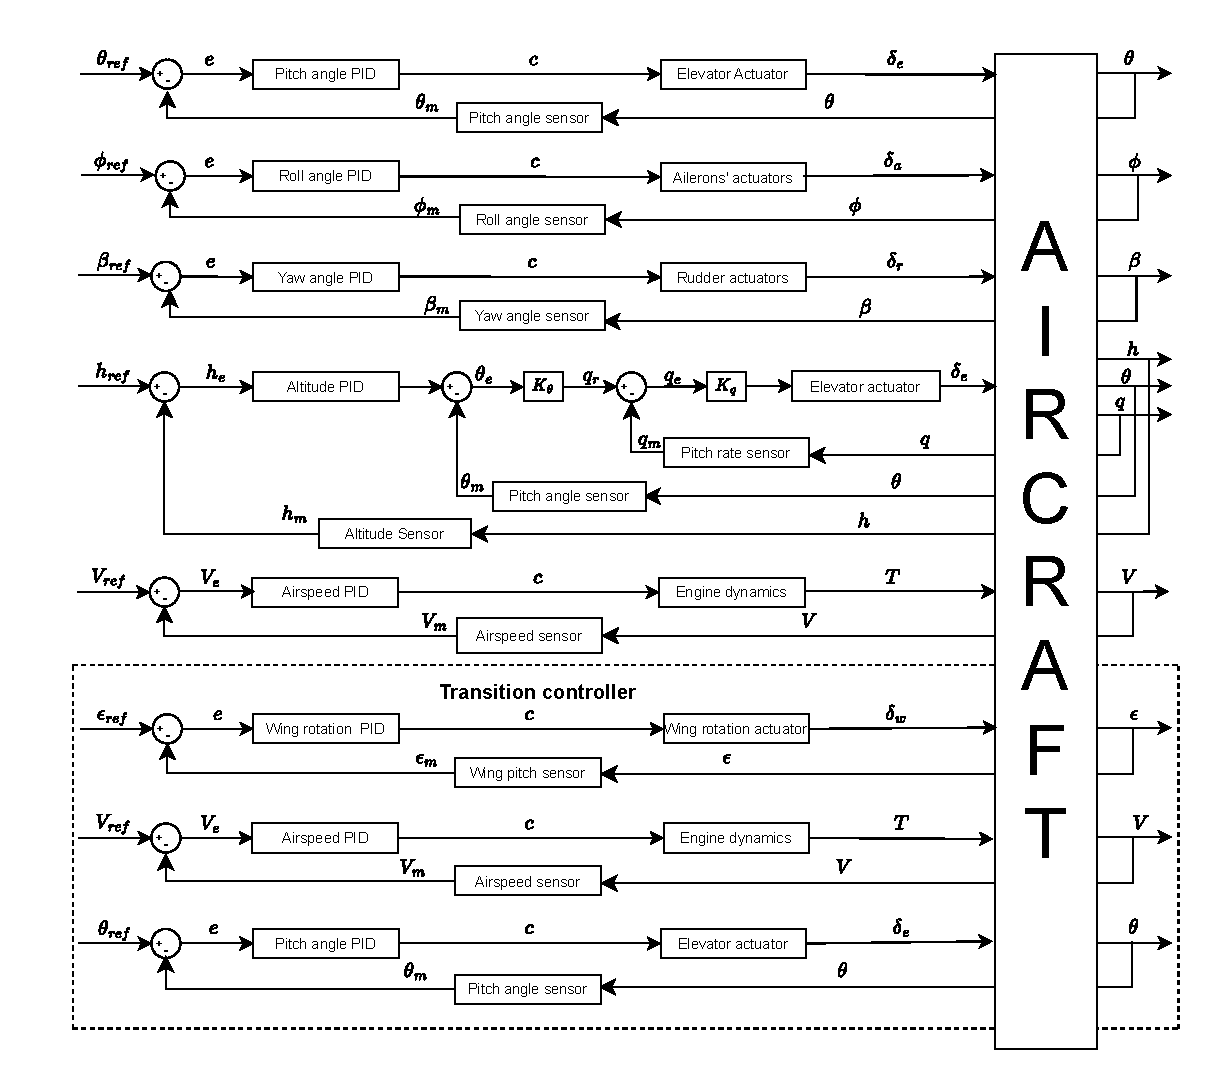
\includegraphics[width=1.0\linewidth]{figures/autopilotV2.pdf}
    \caption{Autopilot block diagram}
    \label{fig: Autopilot}
\end{figure}


\section{Communication Diagram}
\label{sec:CommunicationDiagram}
To understand the flow of data through and from the aircraft system, the communication flow diagram can be used to determine the dependencies between the elements of the communication chain.
Based on literature~\cite{commflow}, the data flow of the design is thus presented below in \Cref{fig:CommFlow}.
As it can be seen in \Cref{fig:CommFlow}, the elements that are part of the communication flow are not necessarily systems of the vehicle, but can also represent external factors such as ground operators.
Additionally, it can be noticed that since the aircraft is autonomous, there is no pilot interface; the air traffic control communicates directly with the autonomous system through the use of transponders placed on the VTOL vehicle.

Subsequently, the flight control computer represents the \enquote{heart} of the communication flow, containing all the relevant information based on which the pilot operates.
Hence, the FCC is the connection between the control part of the aircraft and the sensors and subsystems that the autonomous pilot operates.

\begin{figure}[H]
    \centering
    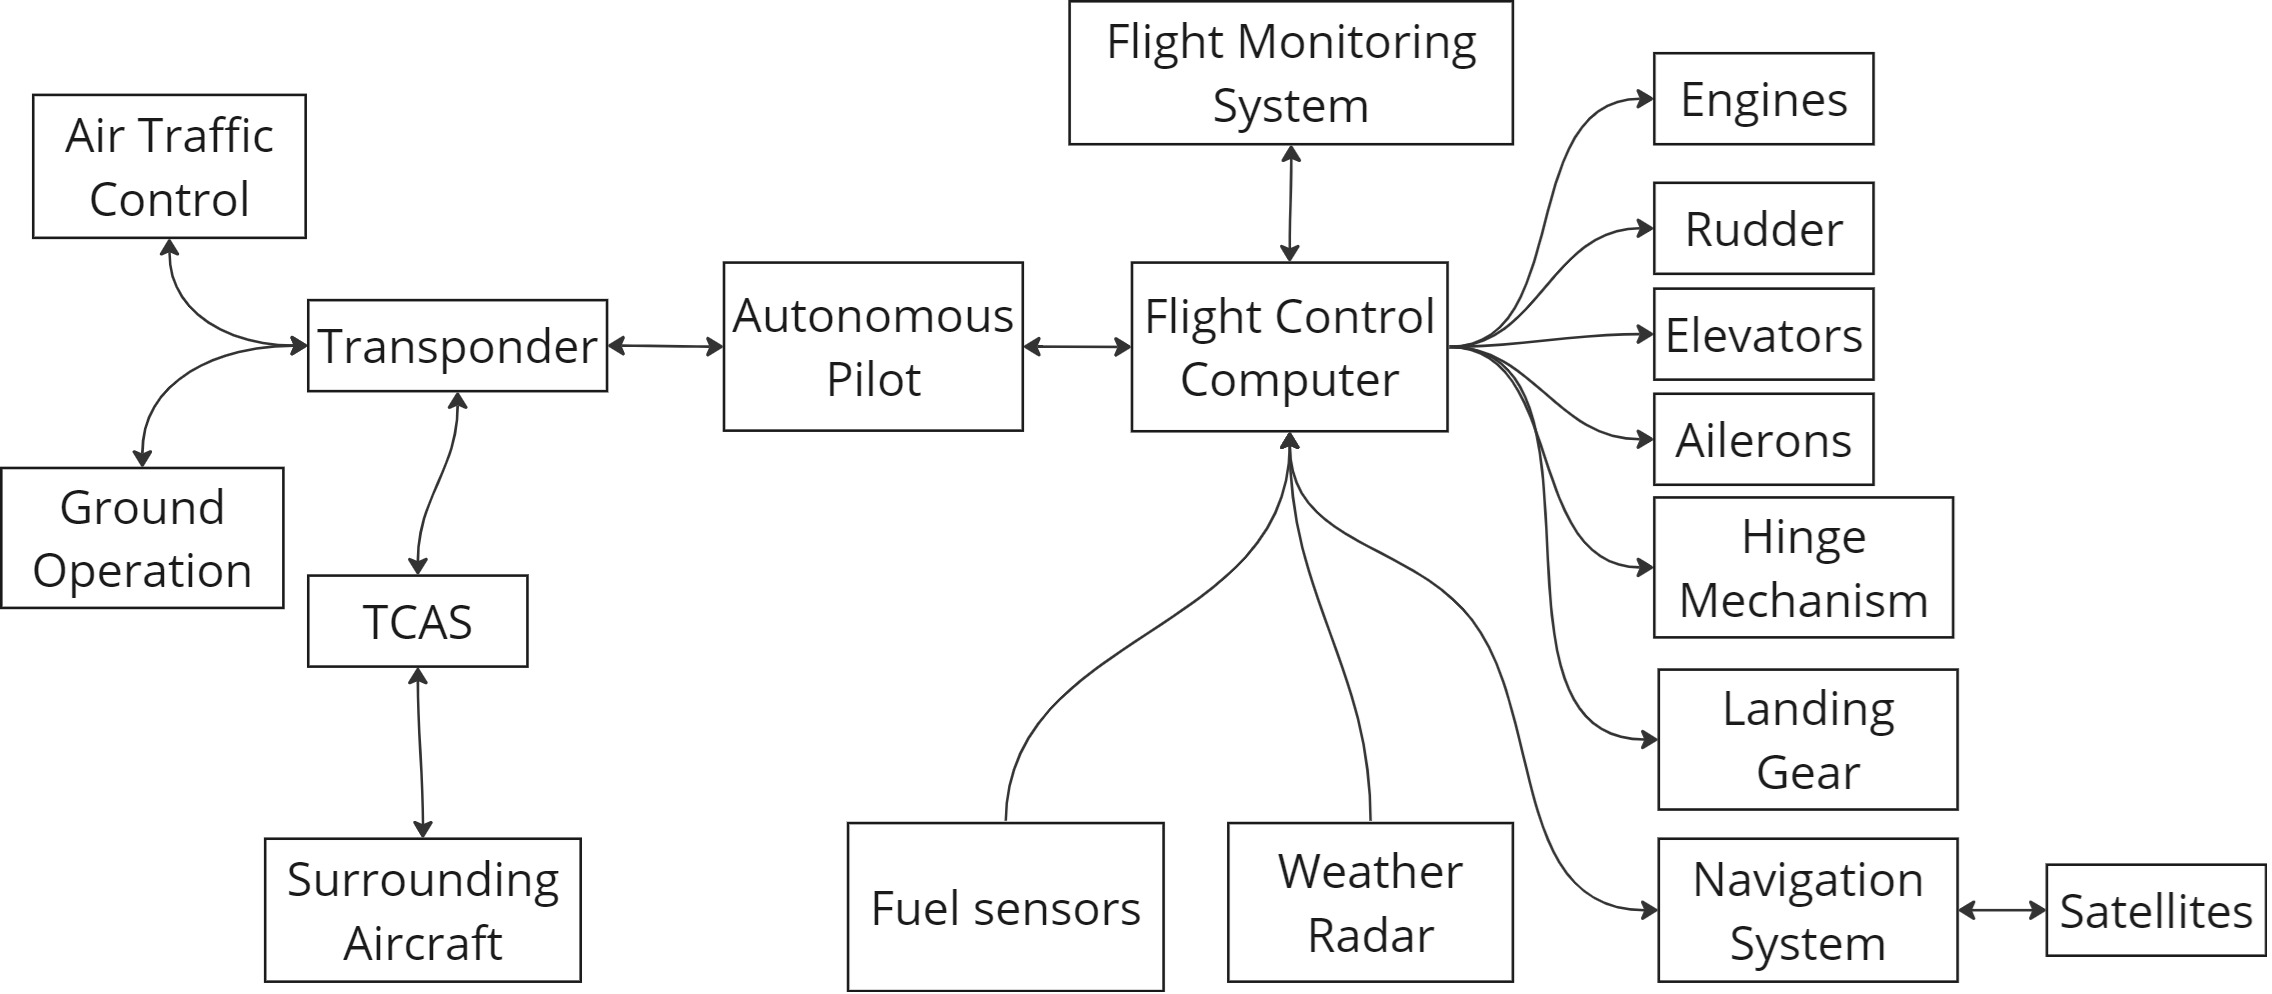
\includegraphics[width=0.9\linewidth]{figures/Communication Flow Diagram.png}
    \caption{Communication flow diagram}
    \label{fig:CommFlow}
\end{figure}
\section{Electric Block Diagram}
\label{sec:ElectricBlockDiagram}
The electrical block diagram shows how all the electrical power is distributed, as the vehicle is electric, all the energy flows from the main battery system, whereas in conventional aircraft it would flow from the turbines or auxiliary power unit.
The main battery bus is split into a high and low-voltage battery pack.
The diagram can be seen in \Cref{fig:Electrical Block Diagram}.

\begin{figure}[H]
    \centering
    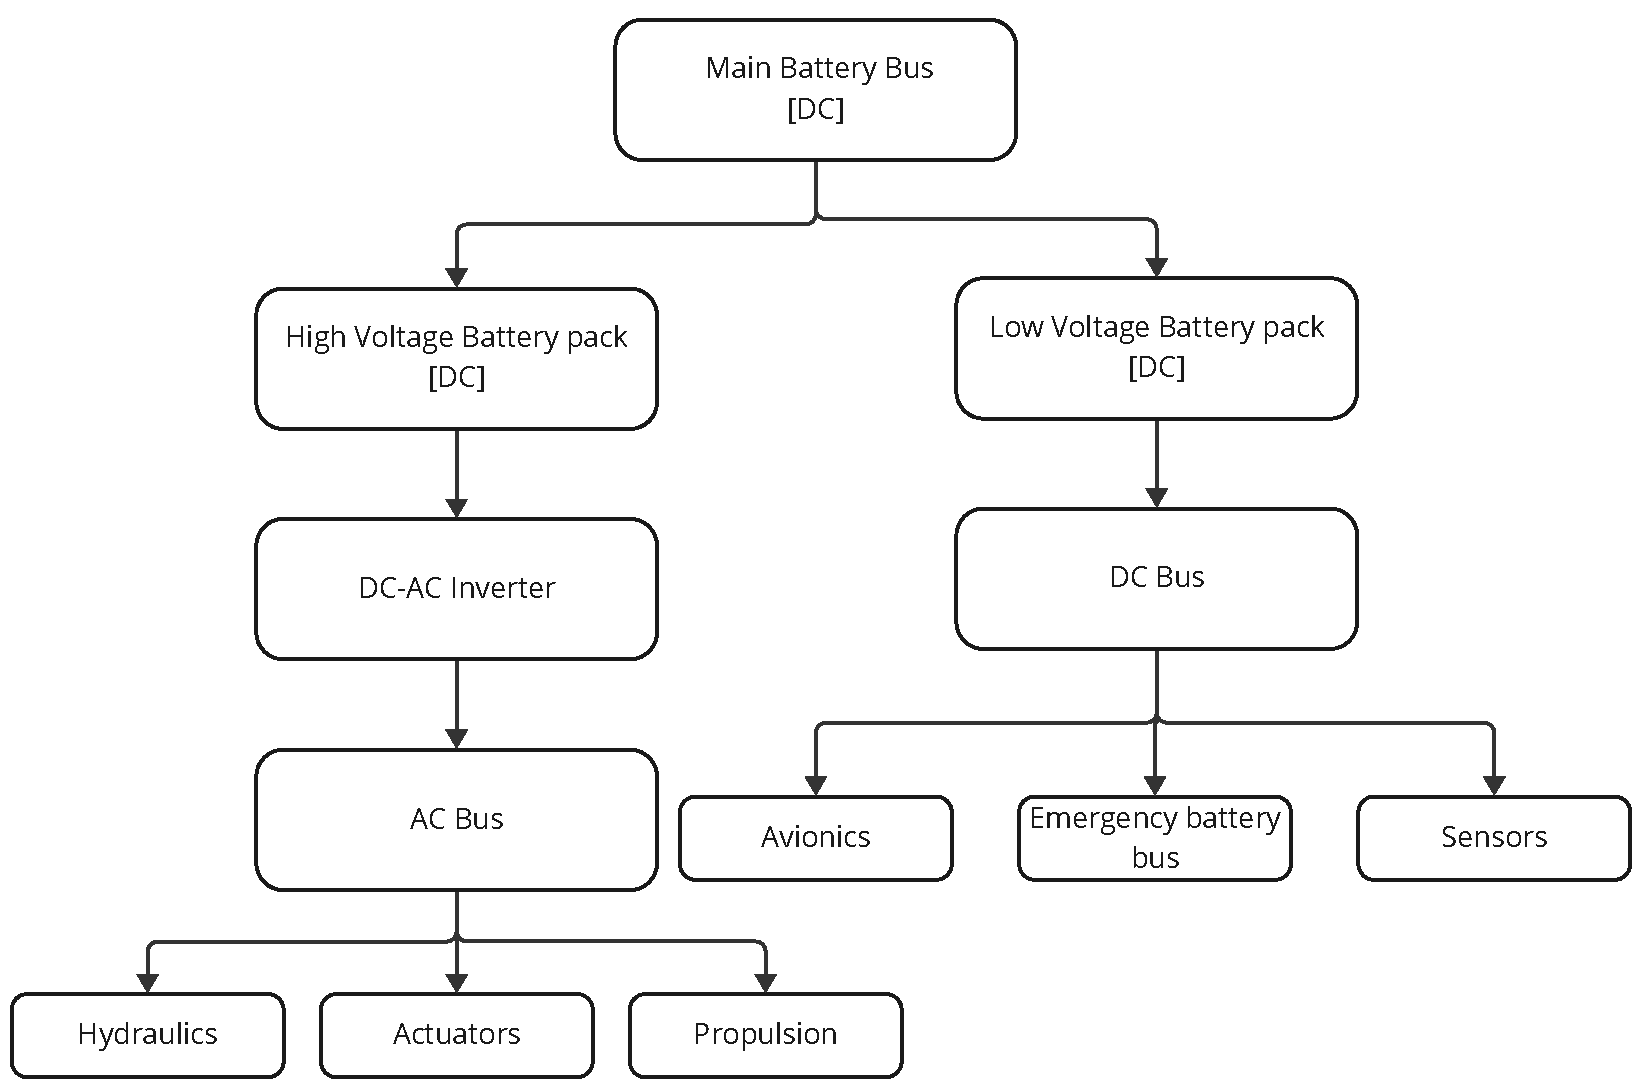
\includegraphics[width=.8\linewidth]{figures/Electrical block diagram (1).pdf}
    \caption{Electrical block diagram}
    \label{fig:Electrical Block Diagram}
\end{figure}

The vehicle battery packs produce direct current both high and low voltages.
The high-voltage DC inverts the direct current into alternating current, which can be used in the AC bus.
The AC bus consists of subsystems that need high voltages, such as the propulsion system.
The DC bus consists of all electrical subsystems that need direct current at a lower voltage, such as the avionics subsystem, which incorporates the autonomous system.
The total overview and how the electric systems are linked can be seen in \Cref{fig:Electrical Block Diagram}.
The emergency battery bus is a low-voltage DC bus since low-voltage DC systems are often used for critical functions that require backup power, such as essential avionics, lighting, and communication systems.
